\chapter{Deep Learning Techniques}
\label{chap:DLTechniques}
%%%%%%%%%%%%%%%%%%%%%%%%%%%%%%%%%%%%%%%%%%%%%%%%%%%%%%%%%%%%%%%
% Outline 
% Introduce Machine Learning, and why traiditonal MLP is not good enough
% 1. Convolutional Neural Networks
% 1.1 Example architecture and sucess in vision tasks
% 1.2 1D CNN implemented on DESI spectra
% 1.3 2D CNN implemented on DESI spectra (Eddies Research)
% 2. Transformers 
% 2.1 Example architecture and sucess in NLP tasks + Vision Tasks --> Connection 
%      to DESI
% 2.2 Multi-Head Attention and Self-Attention for spectral classification
% 2.3 Possilbility of NOT having to k-correct for redshift because of this attention
% 2.4 Adjected ViT architecture for DESI

%%%%%%%%%%%%%%%%%%%%%%%%%%%%%%%%%%%%%%%%%%%%%%%%%%%%%%%%%%%%%%%
\section{Multi-Layer Perceptrons}\label{sec:MLP}

To aid in the classification of supernovae, deep learning techniques can provide 
flexibility and scalability that have been previously unattainable by manual 
methods. The simplest and most widely used architecture in deep learning are feed-forward 
fully connected neural networks, also known as multi-layer perceptrons (MLPs) \parencite{popescu2009}.
These networks are composed of series of ``layers'' of neurons, or nodes, that 
are ``fully connected'' to the previous layer (Figure \ref{fig:MLP}).
Given an input vector $\vec{x}^{(0)}$ with $n$ values, an MLP applies a series of weights to each 
element, resulting in a linear transformation from $\vec{x}^{(0)}$ to $\vec{x}^{(1)}$, where
$\vec{x}_{(1)}$ is a vector of length $m$. This transformation is then followed by a bias added 
to each element, and an activation function applied to each element.
The transition from layer $i$ to $i+1$ can be represented mathematically as 
\begin{equation}\label{eqn:MLP}
    \vec{x}^{(i+1)} = f(\mathbf{W}\vec{x}^{(i)} + \vec{b}^{(i+1)}),
\end{equation}
where $\mathbf{W}$ is an $m \times n$ matrix of weights, $\vec{b}^{(i+1)}$ is a vector of length $m$
representing the bias, and $f$ is the activation function. The activation function can 
be any function, but traditionally they are chosen to be continuous, non-linear, 
monotonically increasing, and differentiable. The most common activation functions 
are the sigmoid function, $f(x_i) = \sigma(x_i) = 1/(1 + e^{-x_i})$, hyperbolic tangent, 
$f(x_i) = \tanh(x_i)$, and the rectified linear unit,
$f(x_i) = \mathrm{ReLU}(x_i) \equiv \max(0,x_i)$, all of which are applied element-wise.
\begin{figure}[t]
    \centering
    \input{tikz/MLP.tex}
    \caption[Diagram of a Multi-Layered Perceptron]{A simple MLP with an input dimension of 4 (green nodes), three hidden layers (blue nodes), and an output dimension of 3 (red nodes). Each node is connected to every 
    node in the previous and next layer. The lines represent the weights, and each 
    node has an associated bias. Figure adapted from \textcite{neutelings2021_nn}.}
    \label{fig:MLP}
\end{figure}
The output layer of the network is a vector tailored for the particular purpose
of the MLP. For example, if the network is used to classify input data $\vec{x}$ into a set of classes, the output is a vector of normalized probabilities of each class. 

The MLP architecture, while simplistic, is very powerful. \textcite{cybenko1989} showed that for any boolean 
function (i.e. 2-class classification), an MLP with a single hidden layer could 
approximate any function arbitrarily well; this is known as the Universal Approximation
Theorem. The theorem is the basis for the success of MLPs in
many fields, but it is also the reason that MLPs are not the best choice for all problems.
MLPs begin to show many complications when training large models, such as the 
exploding/vanishing gradient problem that makes them difficult to train \parencite{nielsen2015}, a lack of invariance under translation (important for many types of data, such as images), 
and exponential growth of the number of trainable parameters \parencite{Naskath2022}. These problems inhibit the use of MLPs on larger datasets and in more complex problems, including 
image recognition, time series analysis, and natural language processing. Since 
the mid-2000s, the weaknesses of MLPs have been addressed by the adoption of 
alternative network architectures such as convolutional neural networks (CNNs) and
transformers.

\section{Convolutional Neural Networks}\label{sec:CNN}
Convolutional neural networks (CNNs) were originally developed
to address the lack of invariance under translation in input data \parencite{fukushima1979}.
CNNs designed for classification are traditionally composed of a series of convolutional layers, 
usually followed by a pooling layer, and a fully connected layer. The convolutional 
layers are composed of a series of filters that take a certain 
number of inputs from the previous layer and apply a kernel to them, resulting in 
a single output. These filters are applied across the entire input space, and are 
commonly referred to as feature maps. 
%Inputs are traditionally padded to preserve 
%the dimensionality of the original tensor size.
If $N$ filters are applied in 
each convolutional layer, the result is a tensor of shape $N\times x$, where 
$x$ is the shape of the original input (which can be 1D or multi-dimensional). 
To reduce the dimensionality of the output, a pooling layer is applied.
The pooling layer takes a certain number of inputs from the previous layer, and 
reduces them to a single output, similar to the convolutional filters, but 
without the kernel application. The most common pooling layer is the max-pooling
layer, which takes the maximum value in each set as the reduced value. 
The process of passing an input through a convolutional filter and pooling layer is shown in Figure~\ref{fig:convolution}. 
These convolution and pooling layers are applied in series until the desired output dimensionality is reached.
\begin{figure}[t]
    \centering 
    \begin{tikzpicture}[
    2d-arr/.style={matrix of nodes, row sep=-\pgflinewidth, column sep=-\pgflinewidth, nodes={draw}}
  ]

  \matrix (mtr) [2d-arr] {
  |[fill=red!30]| 0  & |[fill=red!30]| 0  & |[fill=red!30]| 0  & |[fill=red!30]| 0  & |[fill=red!30]| 0  & |[fill=red!30]| 0 \\
  |[fill=red!30]| 0  & |[fill=orange!30]| 1 & |[fill=orange!30]| 1 & |[fill=orange!30]| 1 &  0 & |[fill=red!30]| 0 \\
  |[fill=red!30]| 0  & |[fill=orange!30]| 0 & |[fill=orange!30]| 1 & |[fill=orange!30]| 1 &  1 & |[fill=red!30]| 0 \\
  |[fill=red!30]| 0  & |[fill=orange!30]| 0 & |[fill=orange!30]| 1 & |[fill=orange!30]| 1 & 0 & |[fill=red!30]| 0 \\
  |[fill=red!30]| 0  & 1 & 1 & 0 & 0 & |[fill=red!30]| 0 \\
  |[fill=red!30]| 0  & |[fill=red!30]| 0  & |[fill=red!30]| 0  & |[fill=red!30]| 0  & |[fill=red!30]| 0  & |[fill=red!30]| 0 \\
  };

  \node[below=of mtr-5-4] {$4\times4$ input with padding};

  \node[right=0.2em of mtr] (str) {$*$};

  \matrix (K) [2d-arr, right=0.2em of str, nodes={draw, fill=teal!30}] {
    1 & 0 &1\\
    0 & 1 &0\\
    1 & 0 & 1\\
  };
  \node[below=of K-2-2] {$3\times3$ filter};

  \node[right=0.2em of K] (eq) {$=$};

  \matrix (ret) [2d-arr, right=0.2em of eq] {
  2 & 2 & 3 &  1\\
  2 & |[fill=blue!80!black!30]| 4 & 3 & 3\\
  2 & 3 & |[fill=orange!30]| 4 & |[fill=orange!30]| 1 \\
  2 & 2 & |[fill=orange!30]| 1 & |[fill=orange!30]| 1 \\
  };
  \node[below=of ret-4-3] {$4\times4$ tensor};

  \node[right=0.2em of ret] (ra) {$\xrightarrow[]{\text{Max Pooling}}$};

\matrix (pool) [2d-arr, right=0.2em of ra] {
  4 & 3 \\
  3 & |[fill=blue!80!black!30]| 4 \\
  };
  \node[below=of pool-2-2] {$2\times2$ tensor};

  \draw[dashed, teal] (mtr-2-4.north east) -- (K-1-1.north west);
  \draw[dashed, teal] (mtr-4-4.south east) -- (K-3-1.south west);

  \draw[dashed, blue!80!green] (K-1-3.north east) -- (ret-2-2.north west);
  \draw[dashed, blue!80!black] (K-3-3.south east) -- (ret-2-2.south west);

  \draw[dashed, blue!80!green] (K-1-3.north east) -- (ret-2-2.north west);
  \draw[dashed, blue!80!black] (K-3-3.south east) -- (ret-2-2.south west);

\draw[dashed, blue!80!green] (ret-3-4.north east) -- (pool-2-2.north west);
  \draw[dashed, blue!80!black] (ret-4-4.south east) -- (pool-2-2.south west);

\end{tikzpicture}

    \caption[Example of a CNN Unit]{A convolutional filter and a $2\times2$ pooling applied to a 2D input. As the filter is passed 
        over the input space, the kernel is applied. The input is padded with zeros to preserve dimensionality, 
        which is then reduced by the max pooling. Figure adapted from \textcite{neutelings2022_conv}.}
    \label{fig:convolution}
\end{figure}

From here, depending on the task, the output of the pooling layer can be fed
into a fully connected layer, similar to the MLP architecture described
in Section~\ref{sec:MLP}, or it can be fed into another convolutional layer. An
MLP is usually applied for classification tasks, while another convolutional layer
is applied for segmentation tasks. An example of a CNN architecture used for 
classification is shown in Figure~\ref{fig:CNN}.

\begin{figure}[t]
    \centering
    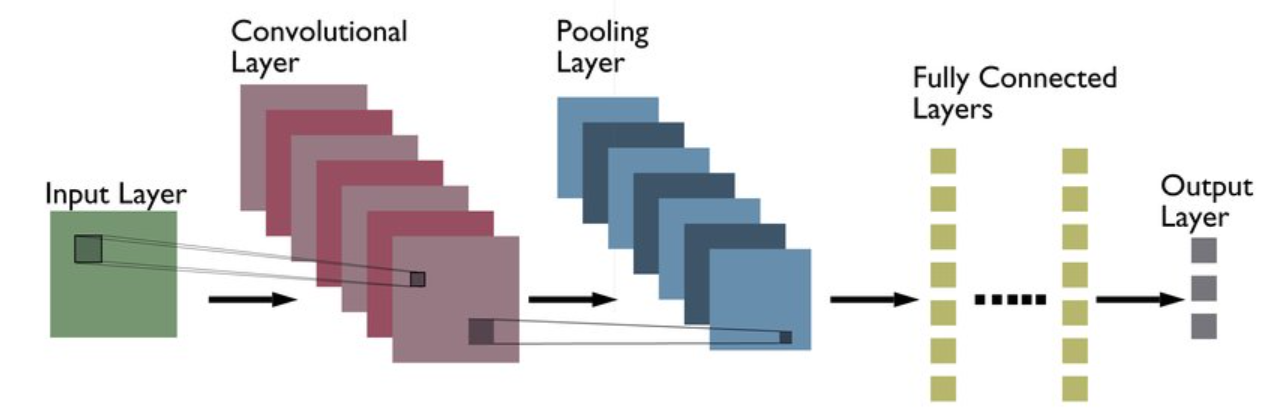
\includegraphics[width=.8\linewidth]{figures/Typical-CNN-architecture.png}
    \caption[Traditional CNN Architecture for Classification]{A convolutional network archeticture designed for classification (adapted from \cite{kumar2022_cnn}). Only
    one convolutional/pooling layer is shown, but there can be multiple depending on the application. }
    \label{fig:CNN}
\end{figure}


The CNN architecture was shown to be effective in image recognition tasks by
\textcite{lecun2004} and then popularized after the success of AlexNet in the 
ImageNet challenge \parencite{krizhevsky2012}. AlexNet was the first of many CNN 
architectures popularized in the 2010s for vision classification, such as VGG~\parencite{Simonyan15}, 
ResNet~\parencite{he2016deep}, and DenseNet~\parencite{Huang2016}. This also spurred a sudden increase in deep networks designed 
for segmentation tasks as well, such as the FCN architecture by \textcite{Shelhamer2016}. In addition to vision tasks, it also found 
great succes in applications such as natural language processing \parencite{Kim2014}, engineering, and 
medicine \parencite{Kiranyaz2021}. 

\subsection{CNNs on Spectroscopic Data in Astronomy}
\label{sec:CNNspectra}
CNNs excel at identifying patterns throughout their input space, stemming from their spacial invariance. 
Theoretically, this should translate to spectral classification quite well. 
Currently running at the National Energy Reserach Scientific Computing Center (NERSC)
is a 1D CNN developed by \textcite{wasserman2021} for DESI transient detection.  This model, while
proven to be effective on training data, is limited by the number of false 
positivies it produces. In order to perform well on DESI data, \textcite{wasserman2021} 
created a preprocessing pipeline that converts the spectra into a format 
that is more easily interpretable by the CNN. This preprocessing pipeline includes 
de-redshifting the spectra into the observed galaxies rest frame, applying a 
log-binning to the spectra, normalizing the flux such that the maximum flux is 1, 
and padding the spectra to a fixed length. 


This work provides a baseline for the use of CNNs on supernovae classification 
which was continued by \textcite{Sepeku2022}, who introduced the use of a
2D CNN for SNe classification, adding a second dimension to the spectra by
re-shaping the spectra from an array of size $N$ to an array of size $N/2\times N/2$. 
The resulting 2D `image' was then fed to a more traditional vision 
CNN architecture (see Appendix~\ref{fig:Sepeku2022_CNN} for a complete diagram of the architecture). 
% TODO: Make into Subcaptions
\begin{figure}[t]
    \centering
    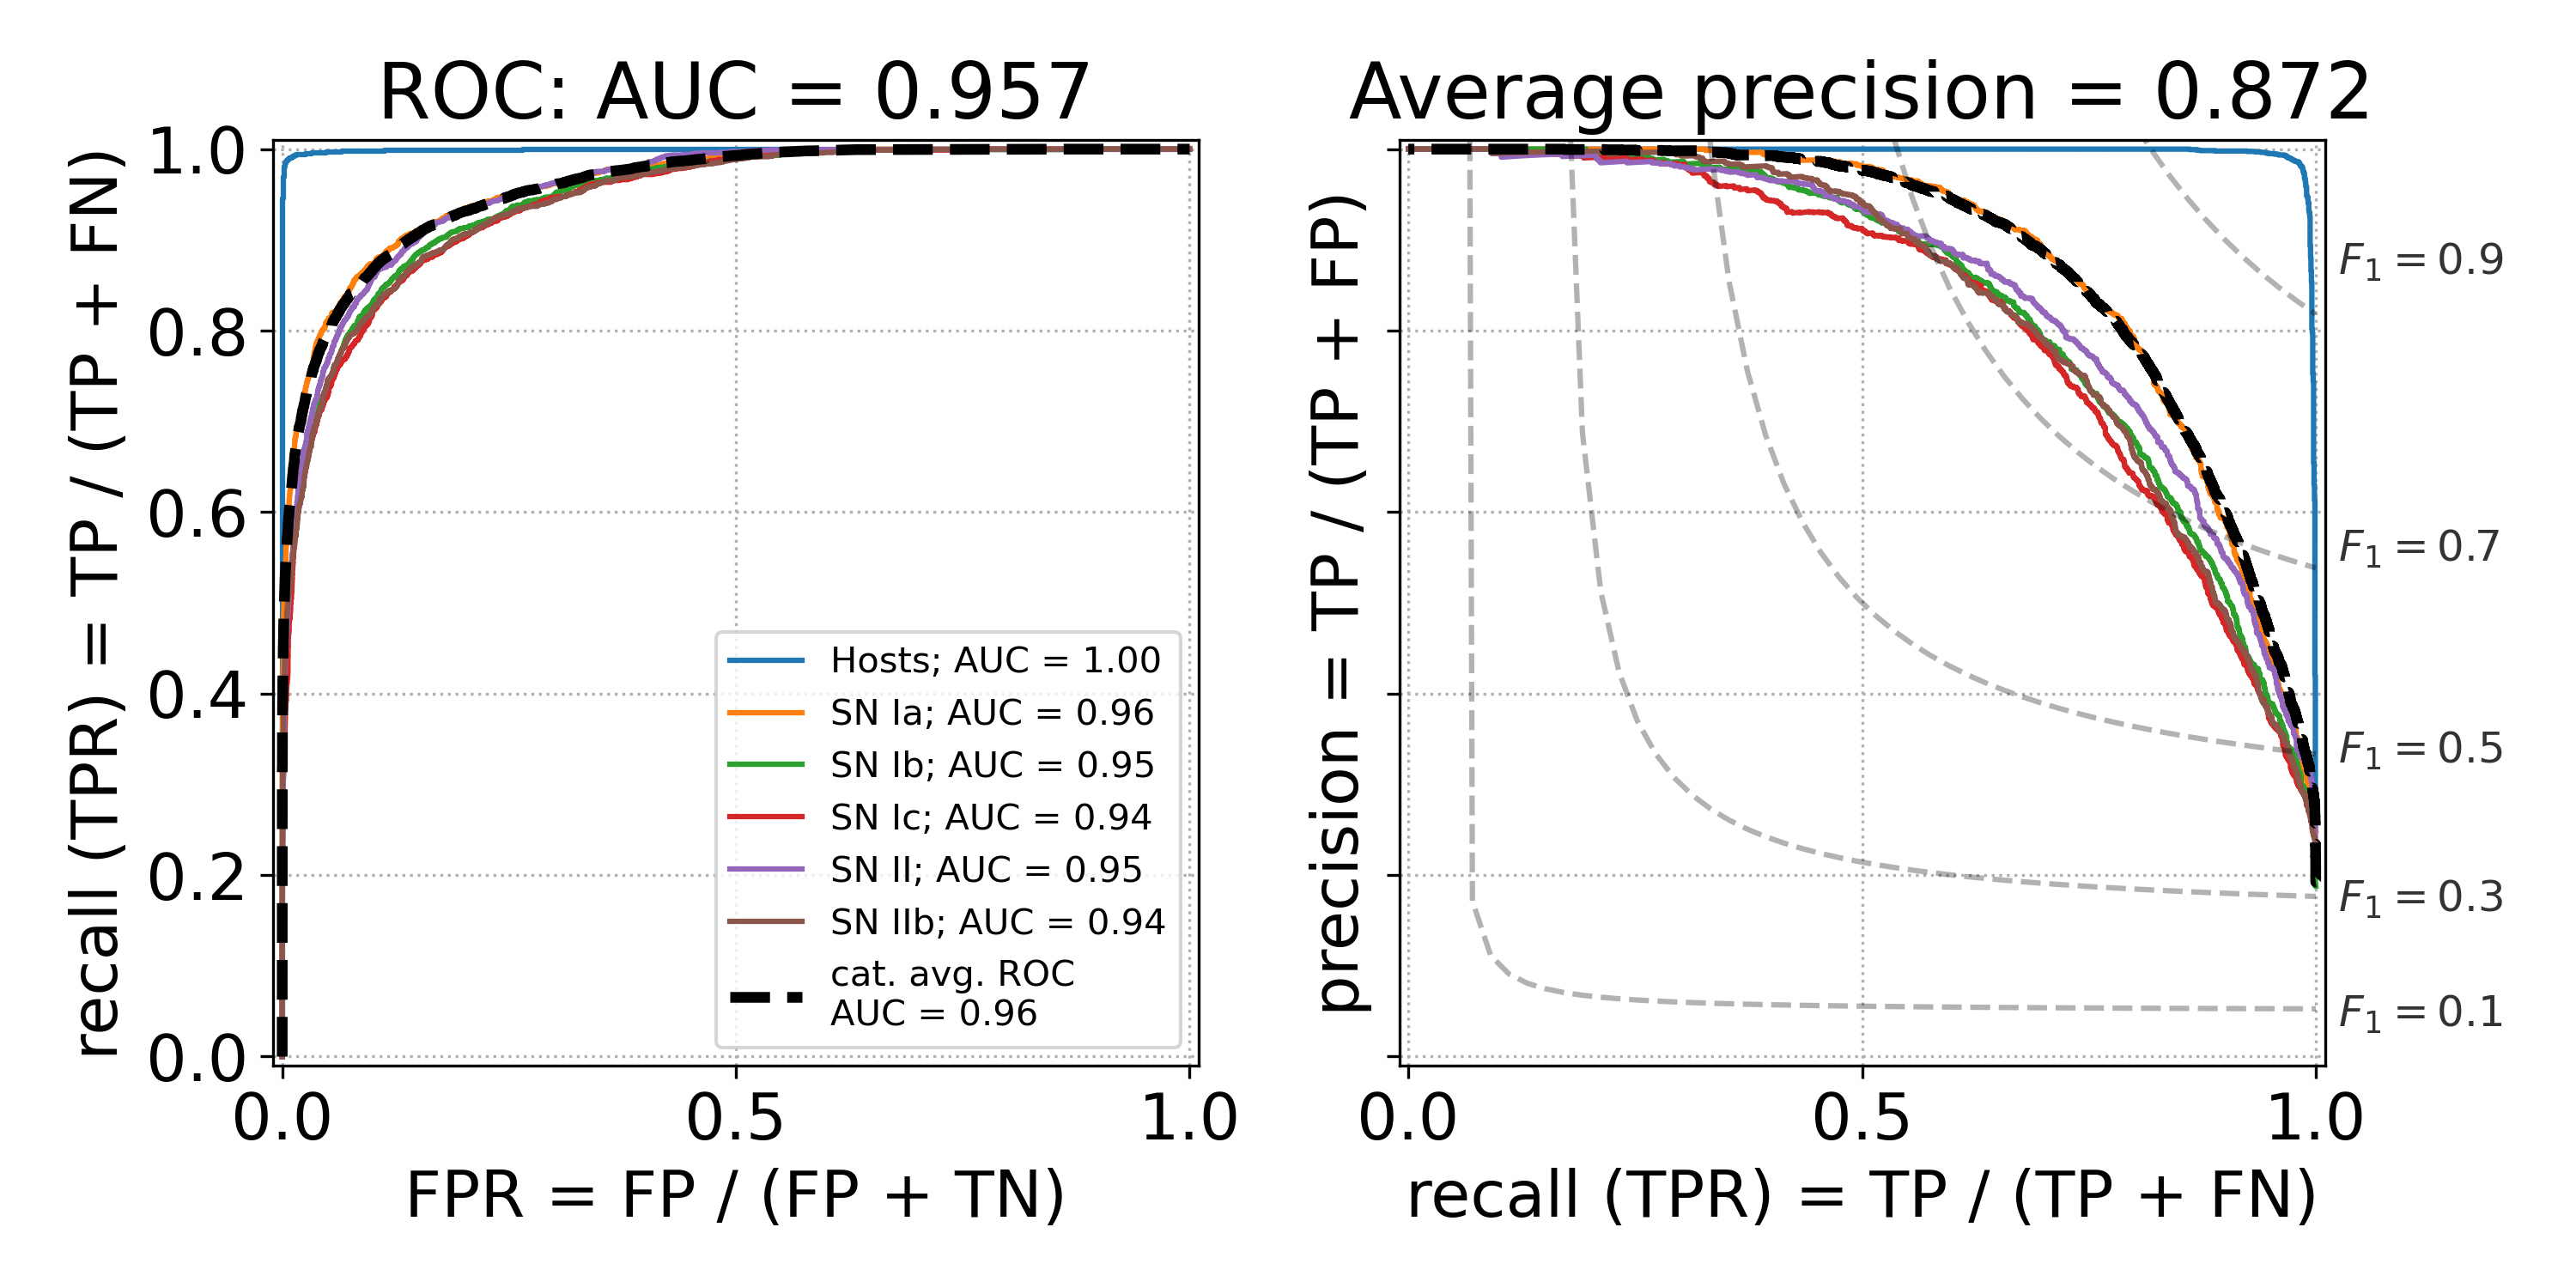
\includegraphics[height=4.55cm]{figures/cnn/cnn_rocfull.png}
    \quad
    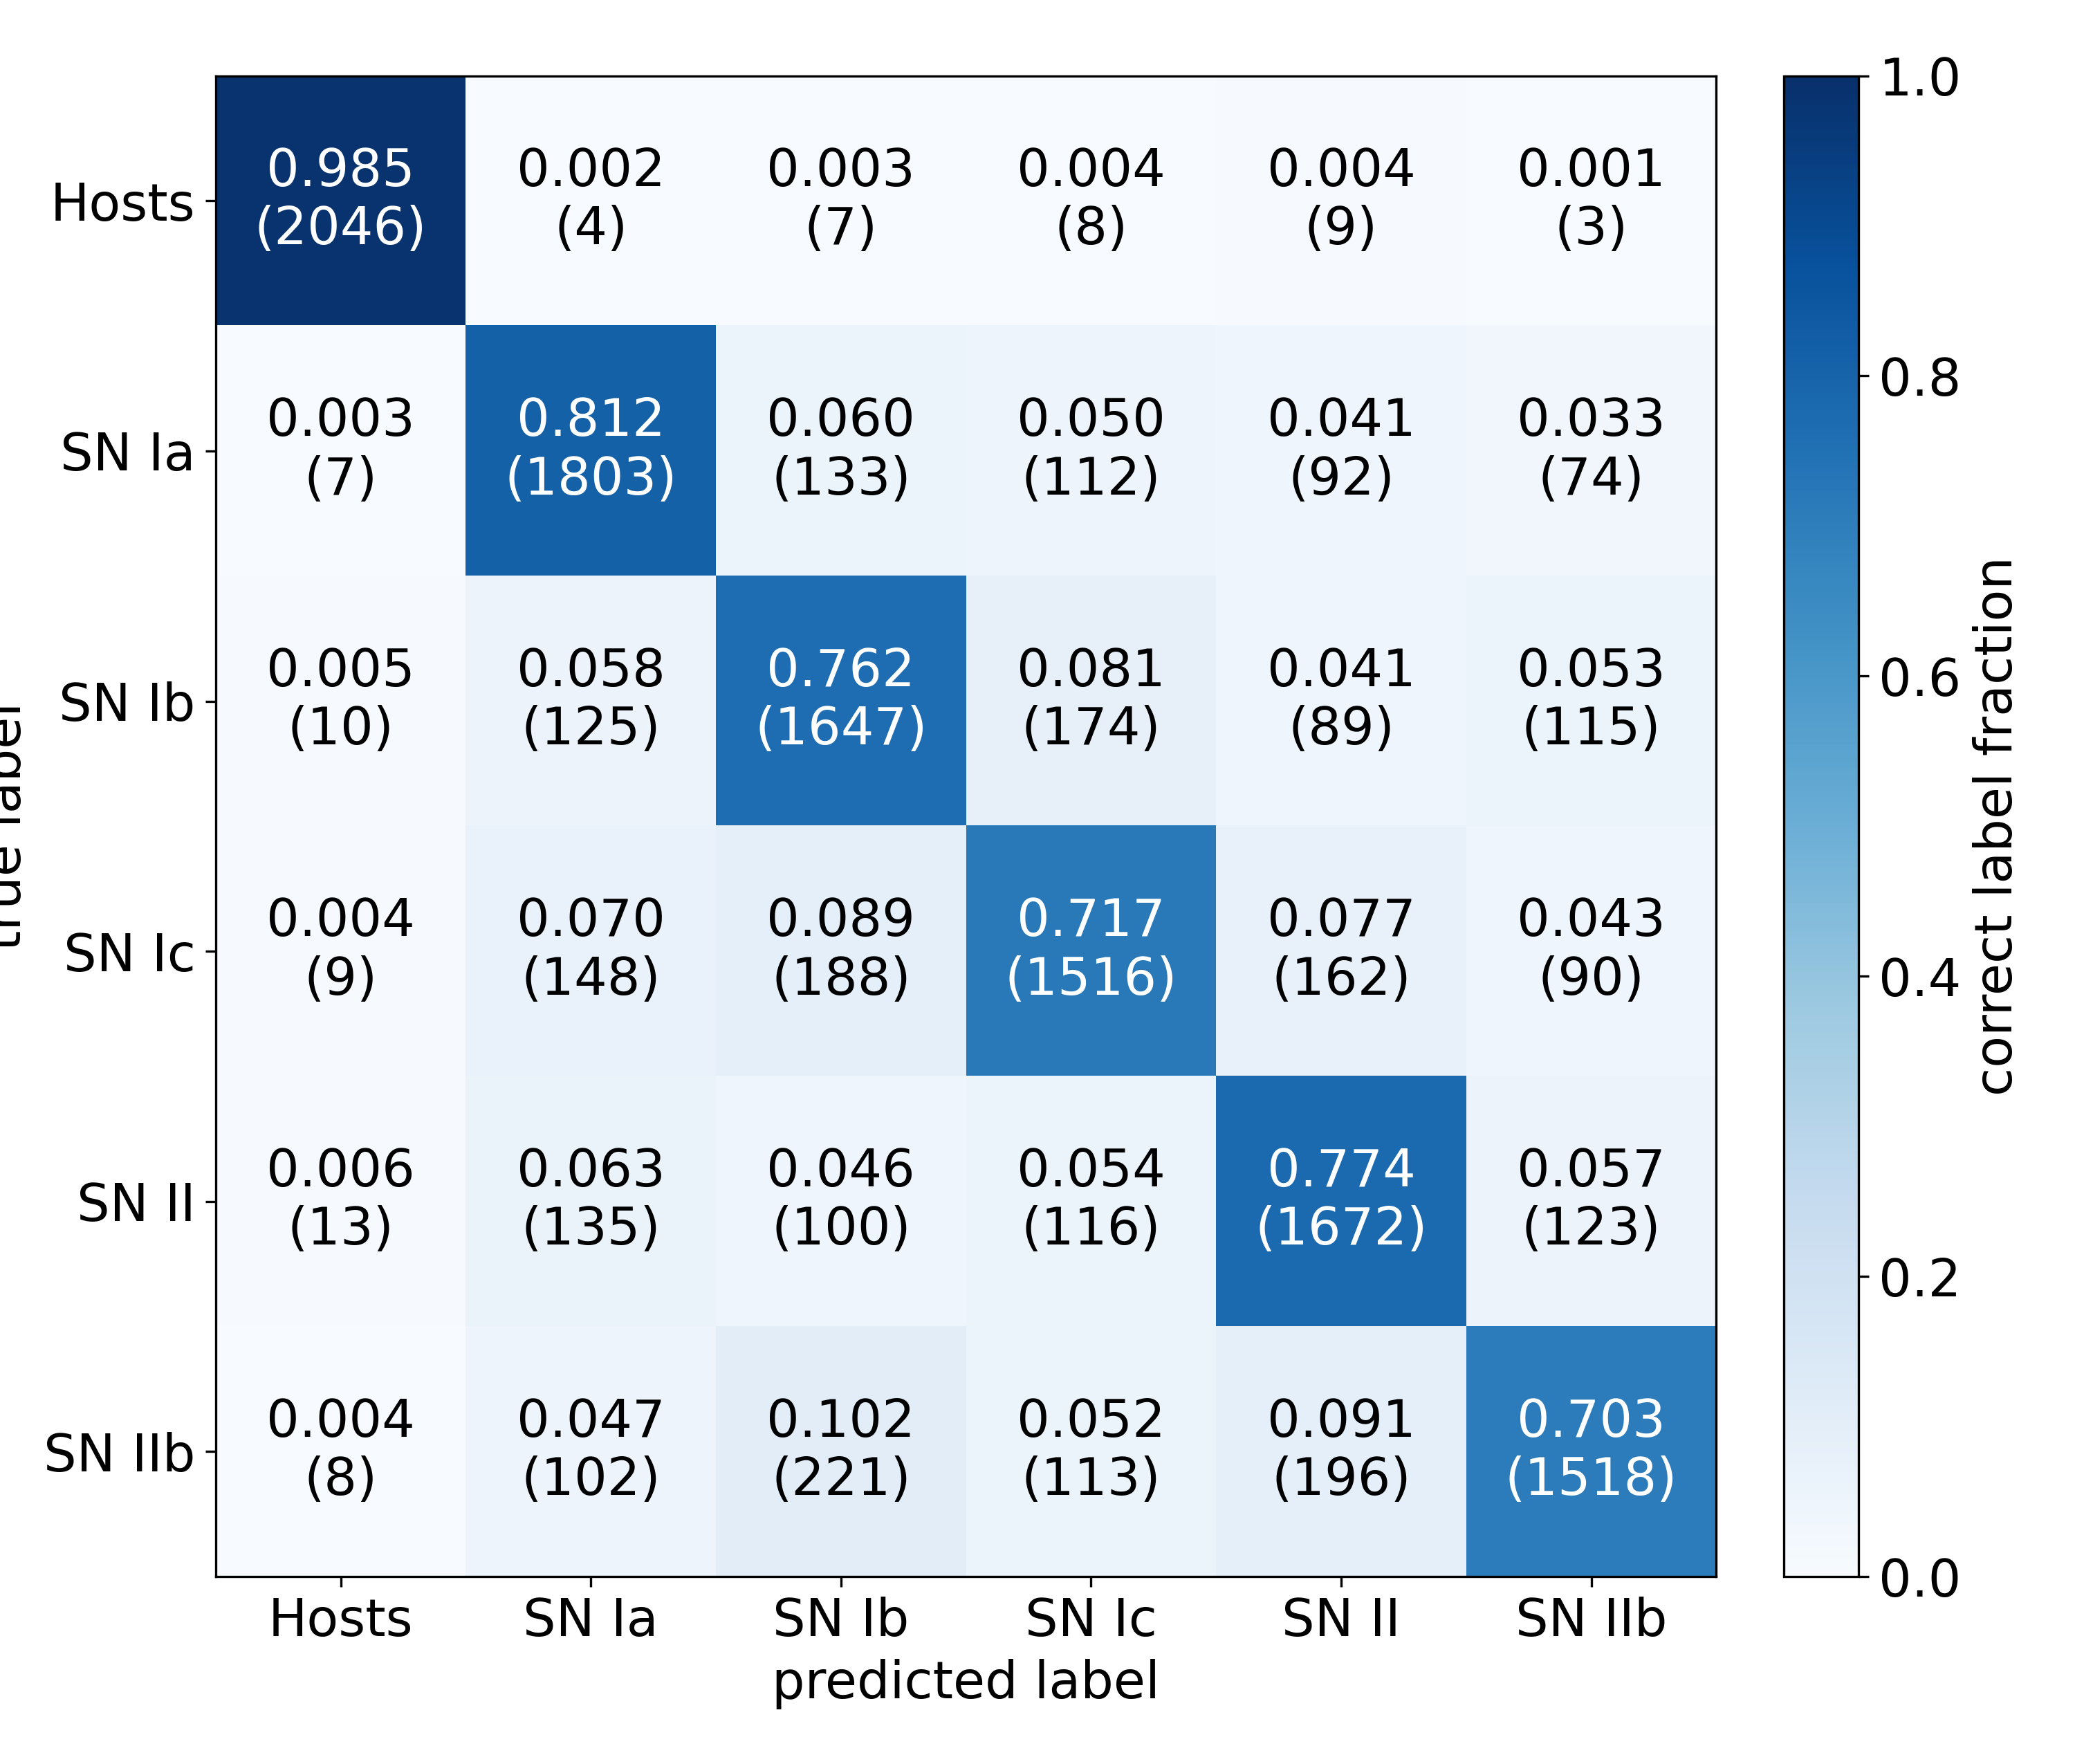
\includegraphics[height=4.55cm]{figures/cnn/cnn_cmfull.png}
    \caption[CNN diagnostics]{CNN Diagnostics: ROC Curve (left) and Confusion Matrix (right)\label{fig:cnn_qual}}
\end{figure}
This architecture was shown to train quickly (less than 1 hour on a single GPU), 
and was able to classify a validation set of 12888 spectra with an average precision of 0.872
via 6-way categorical classification. 

Figure~\ref{fig:cnn_qual} shows the ROC curve and confusion matrix for the 
CNN trained on synthetic spectra. 
\begin{figure}[t]
    \centering
    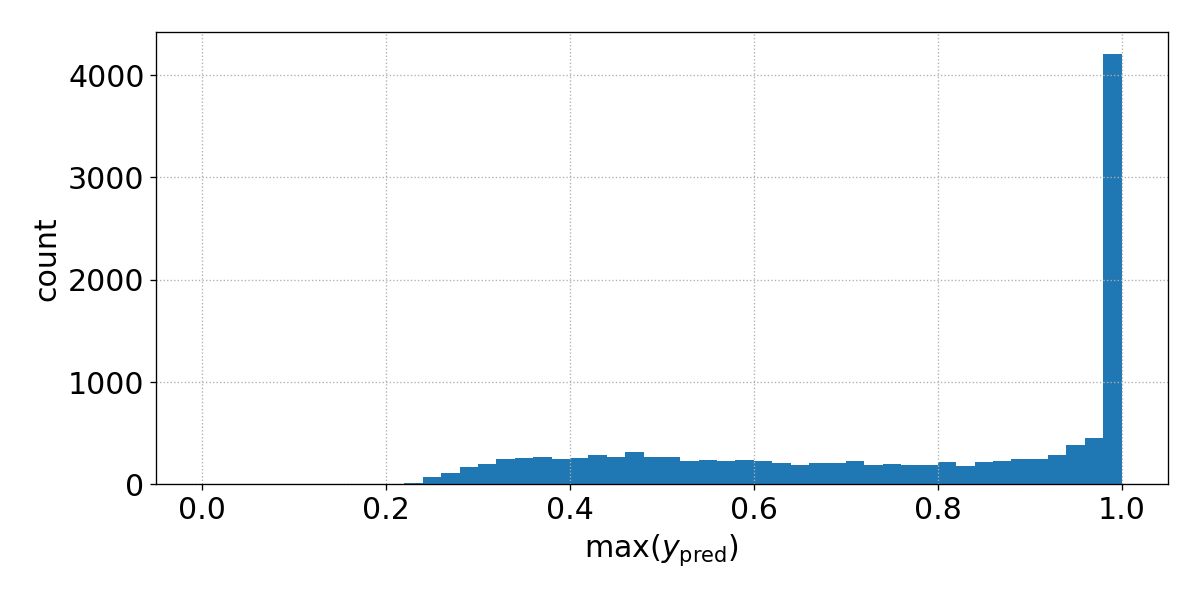
\includegraphics[width=0.6\textwidth]{figures/cnn/cnn_max_ypred.png}
    \caption[CNN's Confidence in Classification]{Max value of the output vector from the CNN.\label{fig:cnn_max}}
\end{figure}

The maximum value of the output vector varied greatly between 1, which indicates a 
confident classification, and 0.2, which indicates a random guess. Figure~\ref{fig:cnn_max} shows
the distribution of the maximum value found. To ensure that the CNN is not
misclassifying spectra with low confidence, a cut on the maximum value of the
output vector can be applied. Figure~\ref{fig:cnn_qual2} shows the ROC curve and confusion matrix
for the CNN trained on synthetic spectra with a 99\% confidence cut, resulting in 
28.8\% of the original validation set. 
% TODO: Make into Subcaptions
\begin{figure}[b]
    \centering
    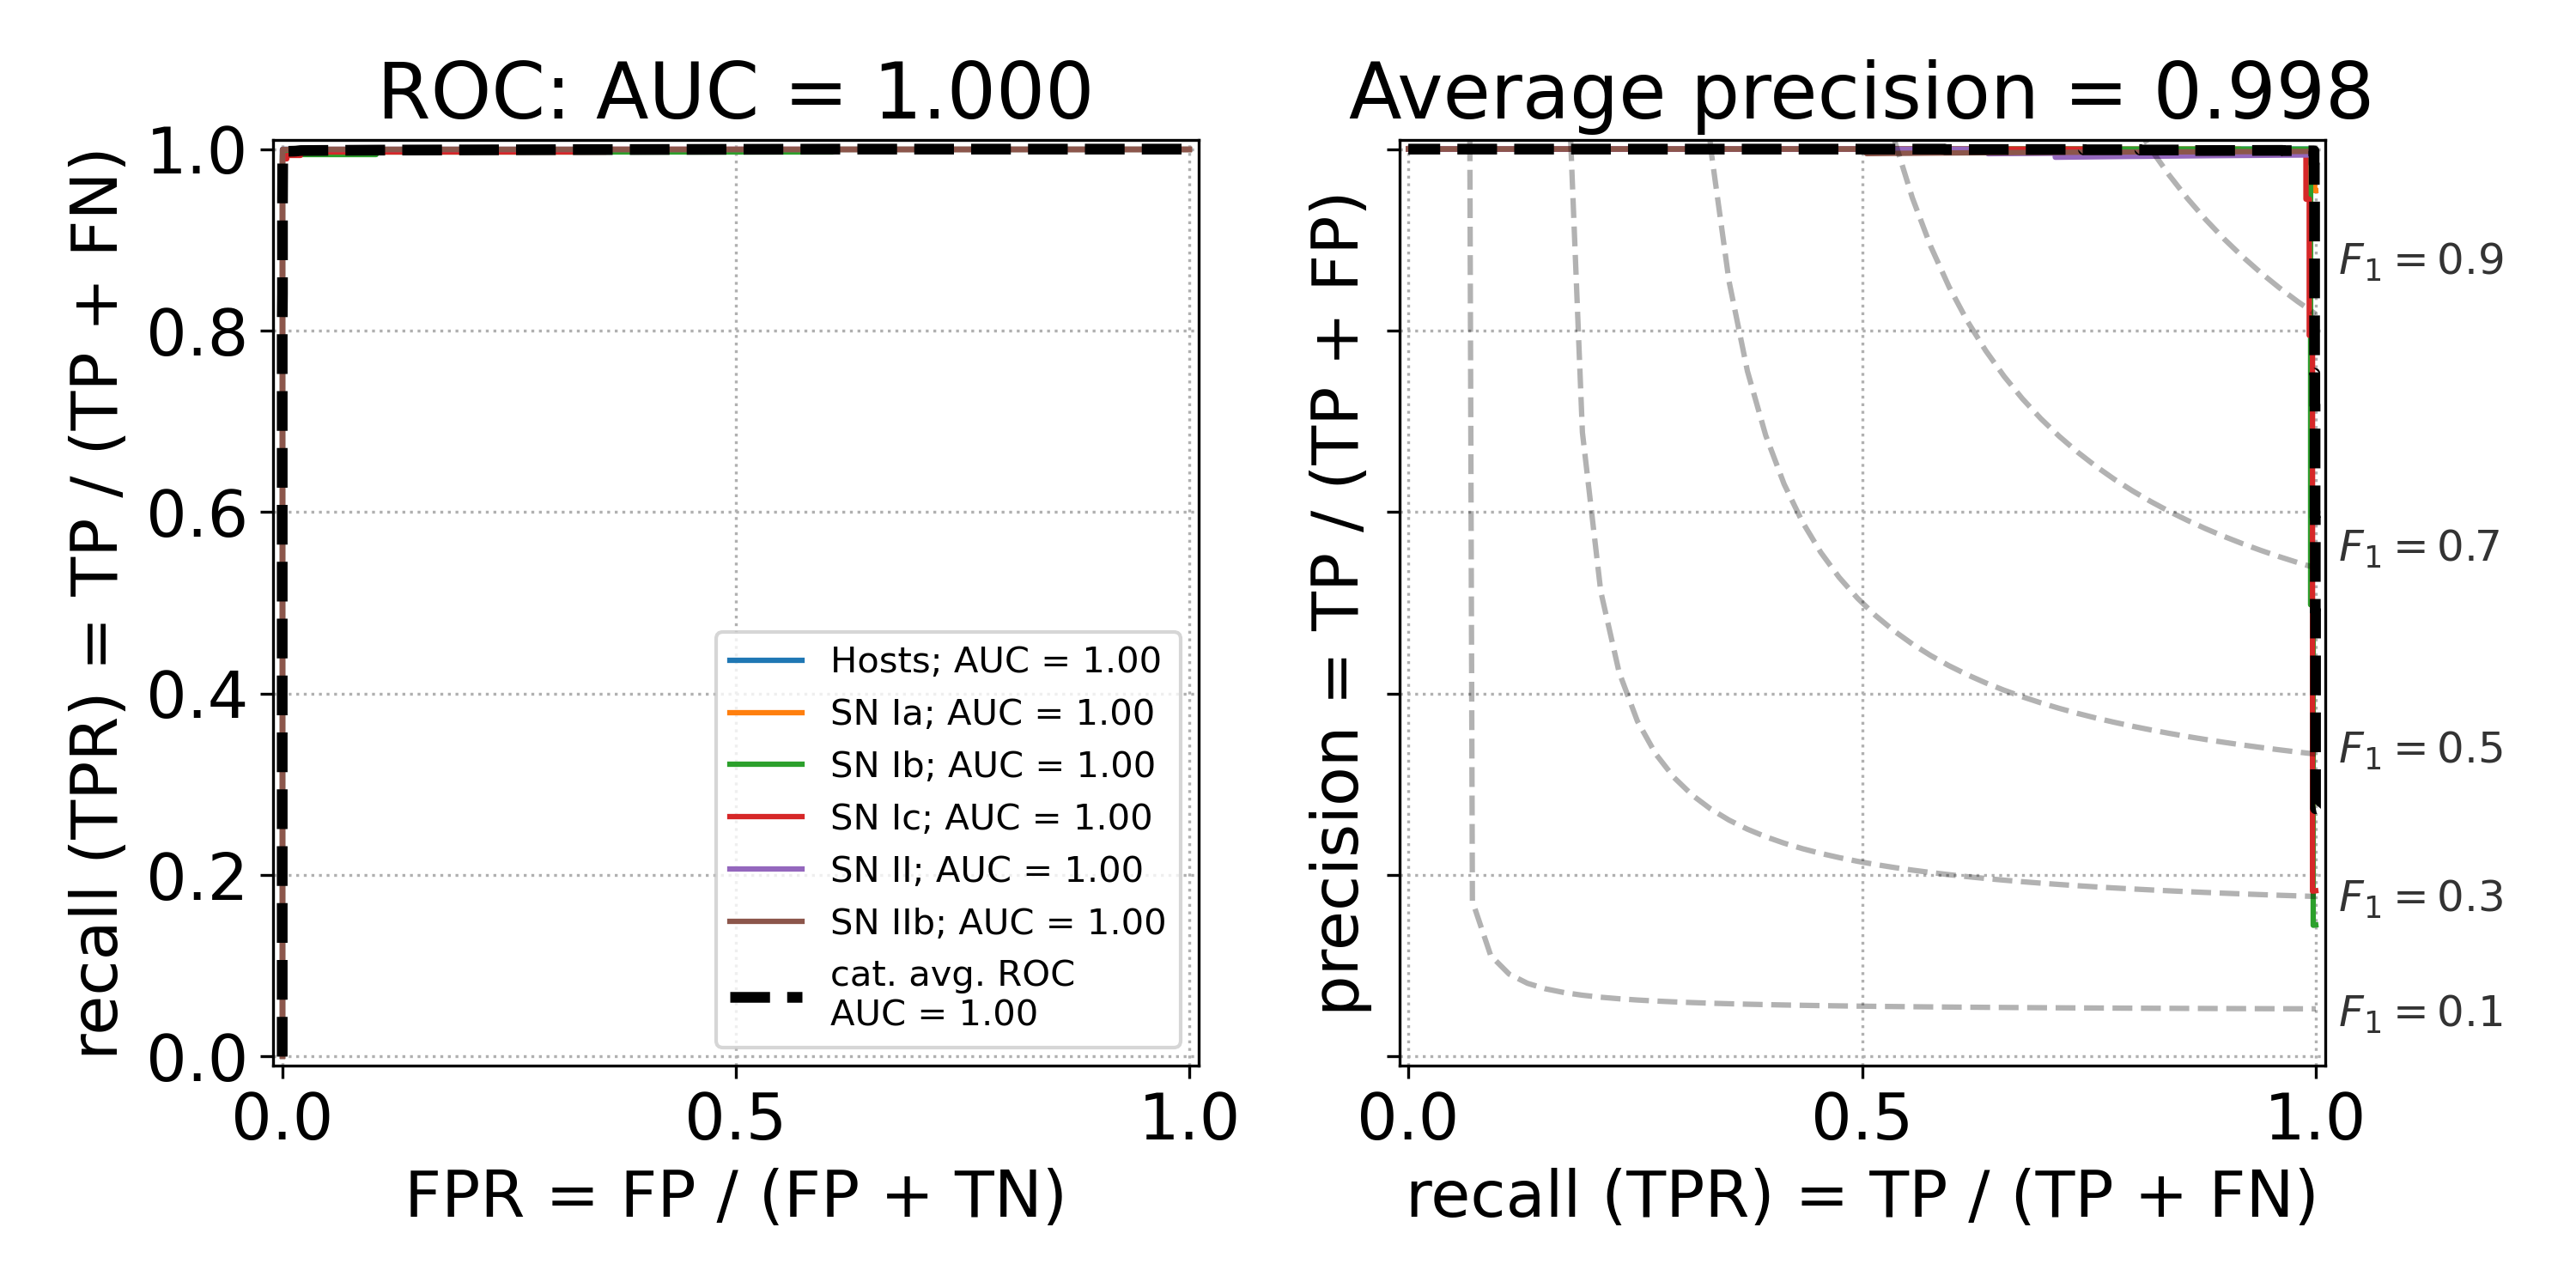
\includegraphics[height=4.55cm]{figures/cnn/cnn_roc99.png}
    \quad
    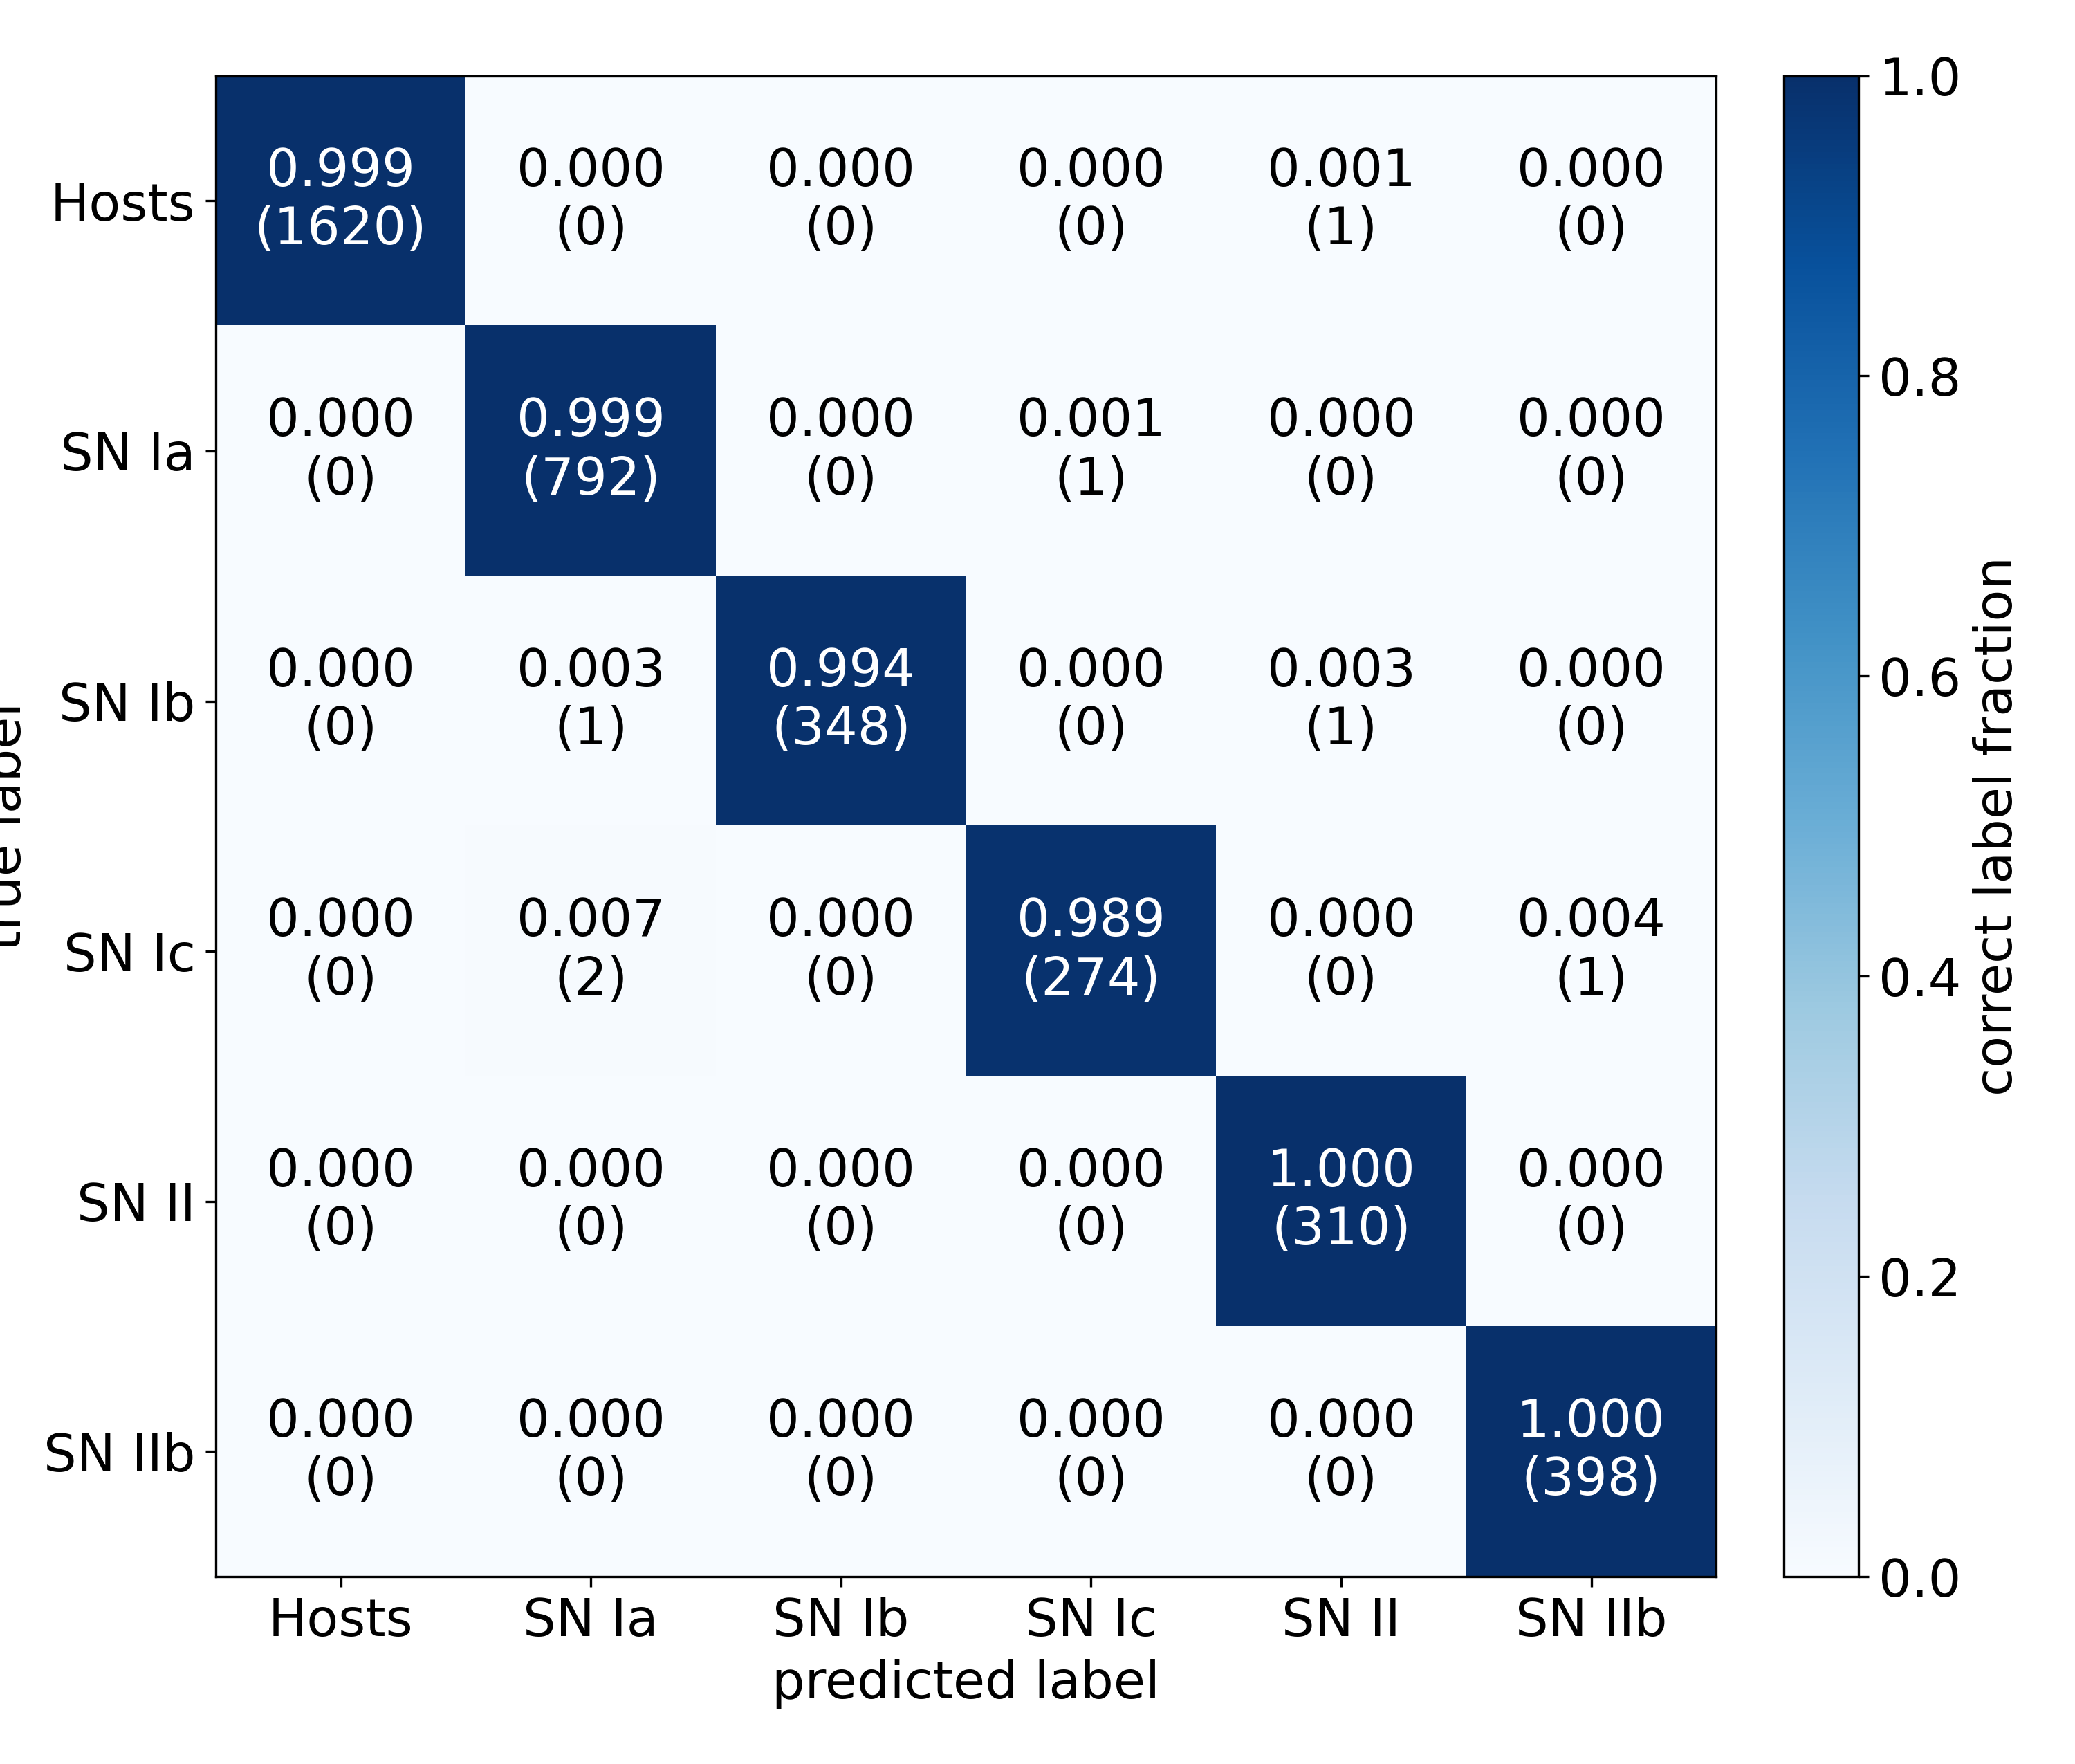
\includegraphics[height=4.55cm]{figures/cnn/cnn_cm99.png}
    \caption[CNN diagnostics with a confidence cut]{CNN Diagnostics: ROC Curve (left) and Confusion Matrix (right) with a 99\% confidence cut\label{fig:cnn_qual2}}
\end{figure}

A nearly perfect ROC curve and confusion matrix are produced by the CNN when
evaluated on only highly confident classifications. This indicates that the CNN
is able to remedy the issue of false positives by only classifying spectra that
it is confident in. However, this cut is not ideal, with only 28.8\% of the
data, sacrificing efficiency for purity.


The next step in training would be to either further increase the accuracy of the CNN 
or move to a different architecture, with the hopes of increasing not only 
the overall accuracy of the networks, but also the number of confident classifications.

\section{From CNNs to Transformers}\label{sec:transformers}
% Advantage of transformers in this field
Transformers are a relatively new architecture introduced in 2017 by \textcite{vaswani2017}
for natural language processing (NLP) tasks. The original architecture consists of 
an encoder-decoder system (Figure~\ref{fig:transformer_orig}). The encoder accepts a series of tokens and produces a series of vectors
representing the input data via a series 
of self-attention layers and feed-forward layers. The decoder then takes the output of the encoder, and
produces a series of output tokens, one for each input token. 

\begin{figure}[ht]
    \centering
    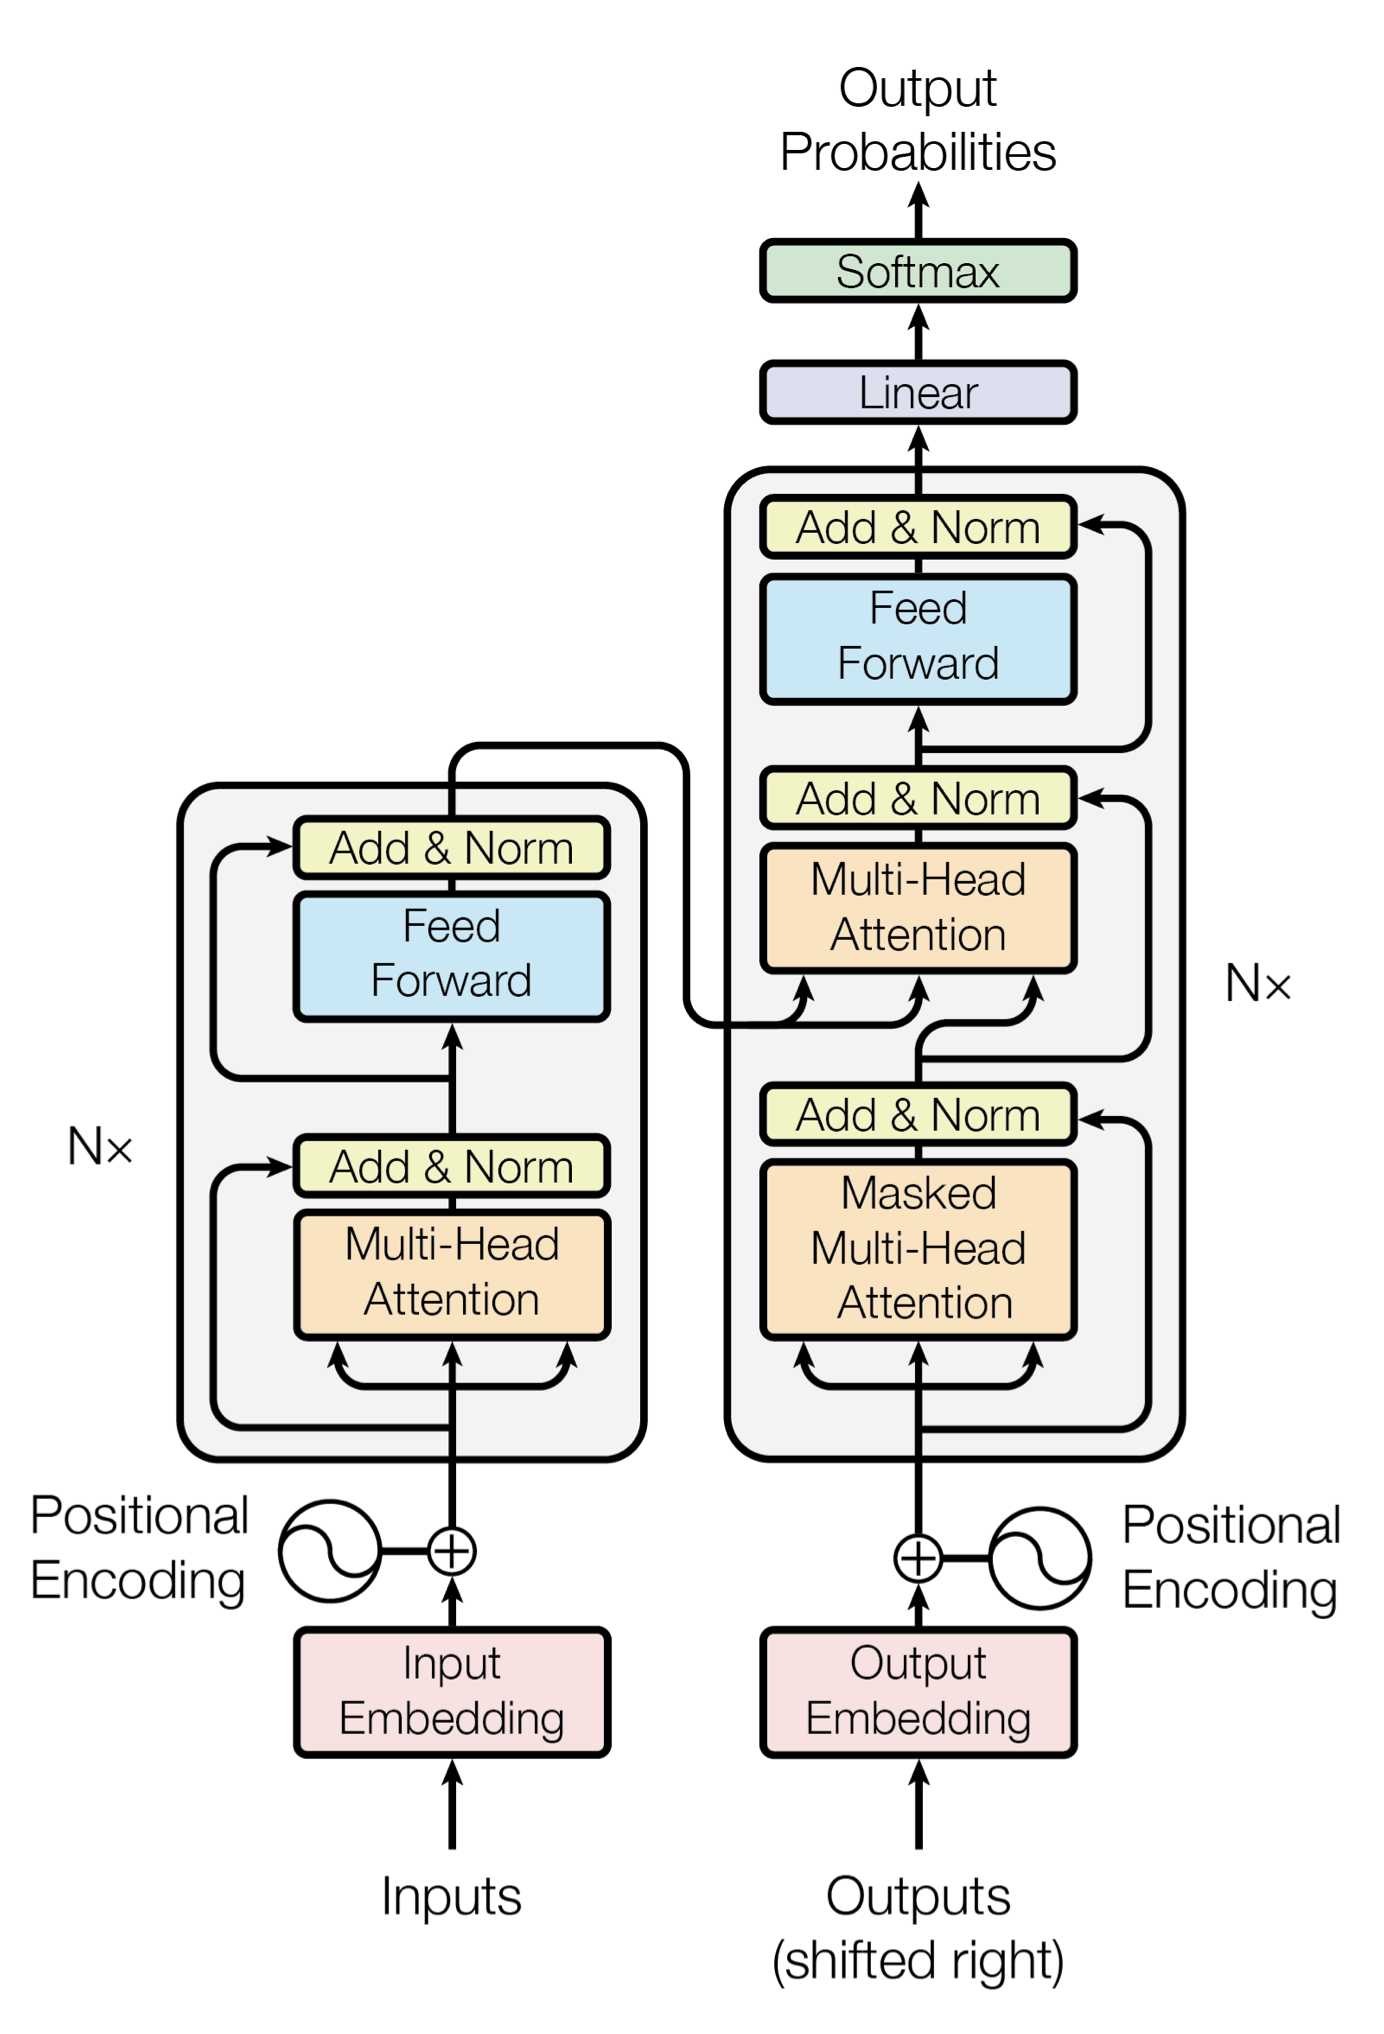
\includegraphics[height=8cm]{figures/transformer_paper/Transformer_Original.png}
    \caption[Transformer Architecture]{Traditional transformer architecture consisting of an enocoder and decoder. 
        Image from \textcite{vaswani2017}
    \label{fig:transformer_orig}}
\end{figure}

Once transformers were shown to have remarkable success in NLP tasks, they were 
quickly adapted to other fields, such as vision and image classification.
\textcite{dosovitskiy2020} developed a vision transformer (ViT) architecture 
that differed from the original transformer encoder by replacing the tokenized 
input with a more image-appropriate alternative. In short, 
the input $n\times n$ image is broken into a series of $m\times m$ patches where 
$m<n$ and $m|n$, which are then flattened into
a vector. These vectors, along with positional encodings, are then fed into the
transformer architecture, as shown in Figure~\ref{fig:ViT_orig}. For classification tasks, the first input token is 
replaced with a class token. After passing through the transformer, the class token 
is then run through a fully connected layer to produce the final categorization probabilities. 
Further details are provided in Section~\ref{sec:SpecViT}. 

\begin{figure}[t]
    \centering
    \includegraphics[width=0.6\textwidth]{figures/transformer_paper/ViT_Original.png}
    \caption[ViT Architecture]{Traditional ViT architecture. Purple ovals indicated 
        positional embeddings, while pink ovals indicate the resulting tokens from 
        the patches. Image from \textcite{dosovitskiy2020}
    \label{fig:ViT_orig}}
\end{figure}

\subsection{ViT on Spectroscopic Data}\label{sec:ViT}
Previous implementations of transformers have been shown to have characteristics 
beneficial to the classification of spectral data. A transformer's 
ability to learn contextual information is essential in spectral classification. 
A broad absorption line, for example, may be indicative of a Type Ia supernova 
if in one part of the spectrum, but may be indicative of a Type II supernova if
in another part of the spectrum. This contextual information is not easily learned 
by a CNN, as the convolutional layers are not able to learn the importance of
certain parts of the input space. Attention can also play a role in identifying 
the purpose of features that are not in a standard location. For example, a 
spectrum in the observers rest frame might have a continuum pattern at different locations 
along the spectrum, but the overall shape would be similar. This change in sizing 
would be difficult to learn with fixed filters in a CNN, but would be identified 
based on their positional importance by a transformer. In addition to this, ViTs 
have been shown to outperform CNNs on vision tasks, which shows they are capable 
of focusing on learned features. 


* Include caveat about the fact that ViTs take longer to train than CNNs *
Very important!!

